
% !TEX encoding = UTF-8 Unicode 
% !TEX root = FieldGuide.tex

\Sec{Laplace Distribution} 
\label{sec:Laplace}
\dist{Laplace} (Laplacian, double exponential, Laplace's first law of error, two-tailed exponential, bilateral exponential, biexponential) distribution~\cite{Laplace1774,Stigler1986,Kotz2001}
 is  a two parameter, symmetric, continuous, univariate, unimodal probability density with infinite support, smooth expect for a single cusp.
The functional form is
\begin{align}
\label{Laplace}
\opr{Laplace}(x\given \pLoc, \theta) = & 
\frac{1}{2 |\theta|} e^{- \Left| \frac{x-\pLoc}{\theta}\Right|} 		\checked
\\
\notag
& \text{for } x,\ \pLoc,\  \theta \text{ in }  \mathbb{R}			\checked
\end{align}
The two real parameters consist of a location parameter $\pLoc$,  and a scale parameter $\theta$.




\SSec{Special cases}
\phantomsection\addcontentsline{toc}{subsection}{~~~~~~~~~~~~Standard Laplace}
The {\bf standard Laplace} (Poisson's first law of error) distribution occurs when $\pLoc=0$ and $\theta=1$.



\SSec{Interrelations}

The Laplace distribution is a limit of the symmetric beta-logistic~\eqref{SymBetaLogistic}, exponential power~\eqref{ExpPower} and generalized Pearson VII~\eqref{GenPearsonVII} distributions.

As $\theta$ limits to infinity, the Laplace distribution limits to a degenerate distribution. In the alternative limit that $\theta$ limits to zero, we obtain an indefinite uniform distribution.


The difference between two independent identically distributed exponential random variables is Laplace, and therefore so is the time difference between two independent Poisson events.
\[
\opr{Laplace}(\pLoc, \theta) \sim  \opr{Exp}(\pLoc,\theta) - \opr{Exp}(\pLoc,\theta)
\notag
\]

Conversely, the absolute value (about the centre of symmetry) is exponential. 
\[
\opr{Exp}(\pLoc, |\theta|) \sim  |\opr{Laplace}(\pLoc,\theta) - \pLoc | +\pLoc
\notag
\]


The log ratio of standard uniform distributions is a standard Laplace.
\[
\opr{Laplace}(0,1) \sim \ln \frac{\opr{StdUniform}_1() }{\opr{StdUniform}_2()} \checked
\notag
\]


The Fourier transform of a standard Laplace distribution is the standard Cauchy distribution \eqref{Cauchy}.
\[
\int_{-\infty}^{+\infty} \frac{1}{2}e^{-| x |} e^{i t x} dx = \frac{1}{1+t^2}
\checked
\notag
\]



\begin{figure}[t!]
\begin{center}
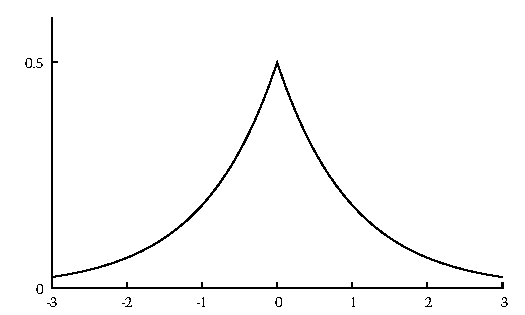
\includegraphics[width=\textwidth]{pdfLaplace}
\end{center}
\caption[Standard Laplace distribution]{Standard Laplace distribution, $\opr{Laplace}(x\given 0,1)$}
\end{figure}


% !TEX encoding = UTF-8 Unicode 
% !TEX root = FieldGuide.tex

\begin{table*}[t!]
\caption[Laplace distribution -- Properties]{Properties of the Laplace distribution}
\begin{align*}
\text{\hyperref[PropertiesSec]{Properties}}  \quad& \\
\text{notation}\quad & \op{Laplace}(x\given \pLoc, \theta) 				\checked
\\ 
\text{PDF} \quad & \frac{1}{2 |\theta|} e^{- \Left|\frac{x-\pLoc}{\theta}\Right|} 	\checked
\\
\text{CDF} \quad & 
\begin{cases}
\phantom{\tfrac{1}{2} -\ } \frac{1}{2} e^{ - \Left|\frac{x-\pLoc}{\theta}\Right| } & x\leq \pLoc  \checked
\\
1 - \tfrac{1}{2} e^{ - \Left|\frac{x-\pLoc}{\theta}\Right| } & x\geq \pLoc 			\checked
\end{cases}
\\
\text{parameters}\quad & \pLoc,\ \theta \text{ in } \mathbb{R}				\checked
\\
\text{support} \quad & x \in [ -\infty, +\infty] 							\checked
\\
\text{median} \quad & \pLoc                            							\checked
\\
\text{mode} \quad & \pLoc 										\checked
\\
\text{mean} \quad & \pLoc  										\checked
\\
\text{variance} \quad & 2\theta^2 									\checked
\\
\text{skew} \quad & 0 											\checked
\\ 
\text{kurtosis} \quad & 3 											\checked
\\ 
\text{entropy} \quad & 1+ \ln( 2 \theta) 								\checked
\\ 
\text{MGF} \quad &  \frac{\exp(\pLoc t) }{1- \theta^2 t^2}					\checked
\\
\text{CF} \quad & \frac{\exp(i\pLoc t) }{1+ \theta^2 t^2}					\checked
\end{align*}
\end{table*}
